\section{Flow correlations}
\label{sec:ps:flow}
%5. Flow Correlations & Flow & PID Flow (PS)
%- Geometric fluctuations and origin of v_n vs ecc_n (Glauber, v3)
%- non-PID flow (ALICE first results)
%- PID flow (ALICE v2 scaling)
%- 2PC (CMS v_n?)
%- Event plane (ATLAS EP)
%- Explaining the ridge (2PC from 3 experiments)
%- Flow fluctuations
%- Event plane correlations
%- Success of viscous hydro
%- Comparison with RHIC
%- Flow in p+Pb (ridge, double ridge, PID)
%- Open questions

While the previous section covered physical mechanisms which induce
correlations between multiple hadrons, this section covers the
phenomenon of ``collective flow'', which leads to the correlations of
essentially all the particles in every event.
This results from the translation of anisotropies in the initial shape of the
colliding nuclei into anisotropies in momentum space, something that
would not occur if individual nucleon-nucleon collisions emitted independently
of each other.
The characterization of a ``shape'' in a final state particle distribution
is typically performed using a Fourier decomposition of the azimuthual
angle distrbution of final state particles.
Of course, averaging over an ensemble of independent events would lead to
the observation of no net anisotropy.  Thus, the presence of harmonic
oscillations in the final state requires the estimation of an ``event plane''
from the particle themselves, with an axis that points in the direction of
the largest momentum flow.

While this phenomenon was observed decades ago in the collisions of large
nuclei at low energies, this was straightforward to understand as the
reinteraction of the initial baryons and the produced hadrons, which
would thermalize and evolve as a ``hadron gas''.  
However, its persistence at higher energies, particularly at RHIC where the
value of $v_2$ averaged over \pT was twice as large as it was at the 
CERN SPS, surprised many who expected the hot system to become more
dilute and more weakly-interacting at higher energies.

Collective flow was a major piece of the RHIC program, and its characterization
in terms of hydrodynamics was a crucial piece of evidence in the RHIC discovery
of the strongly-coupled quark gluon plasma (sQGP).  Crucial aspects of collective
flow, on the experimental and theoretical sides at RHIC, have been:
\begin{itemize}
\item Based on theoretical calculations, the average elliptic flow, scaled by the eccentricity, 
is thought to reach a limiting value in the limit where
the viscosity can be ignored.  RHIC data achieved this limit both integrally (integrated over \pT)
and for $v_2(\pT)$, which rises linearly until viscous corrections become large.
\item When studied as a function of particle type, it is found that heavier particles show
a smaller $v_2$ at the same \pT at low \pT, while this hierarchy flips above 1.5 GeV, where protons
typically have a 50\% higher value of $v_2$.  This behavior has been explained by the hadronization of
the system via constituent quarks which recombine into baryons with $v_2$(baryon)=$(3/2) \times v_2$(meson).
\item The deviations from ideal behavior can be systematically calculated by viscous corrections, and
all RHIC data point to a small but significant value of the ratio of shear viscosity to entropy density ($\eta/s$).
\item While difficult to calculate in the strongly-coupled limit, where the approximations required for kinetic theory break down, AdS/CFT-based calculations have shown that a wide range of strongly-coupled systems have a lower-bound on 
$\eta/s = 1/4\pi$.  The RHIC experimental data suggest values of 1-2 times this bound, although esimates are limited
by theoretical uncertainties related to the modeling of the initial state.
\item When studying smaller systems (particularly Cu+Cu), it was found that accounting for the event-by-event position of the nucleons in the nuclear wave functions showed scaling in the quantity $v_2/\epsilon$ between Cu+Cu and Au+Au, when
plotted as a function of the transverse density of charged particles at mid-rapidity, estimated by $dN_{ch}/d\eta/S$,
where $S$ is the overlap area of the two nuclei.
\end{itemize}

\begin{figure}[!htb]
\begin{center}
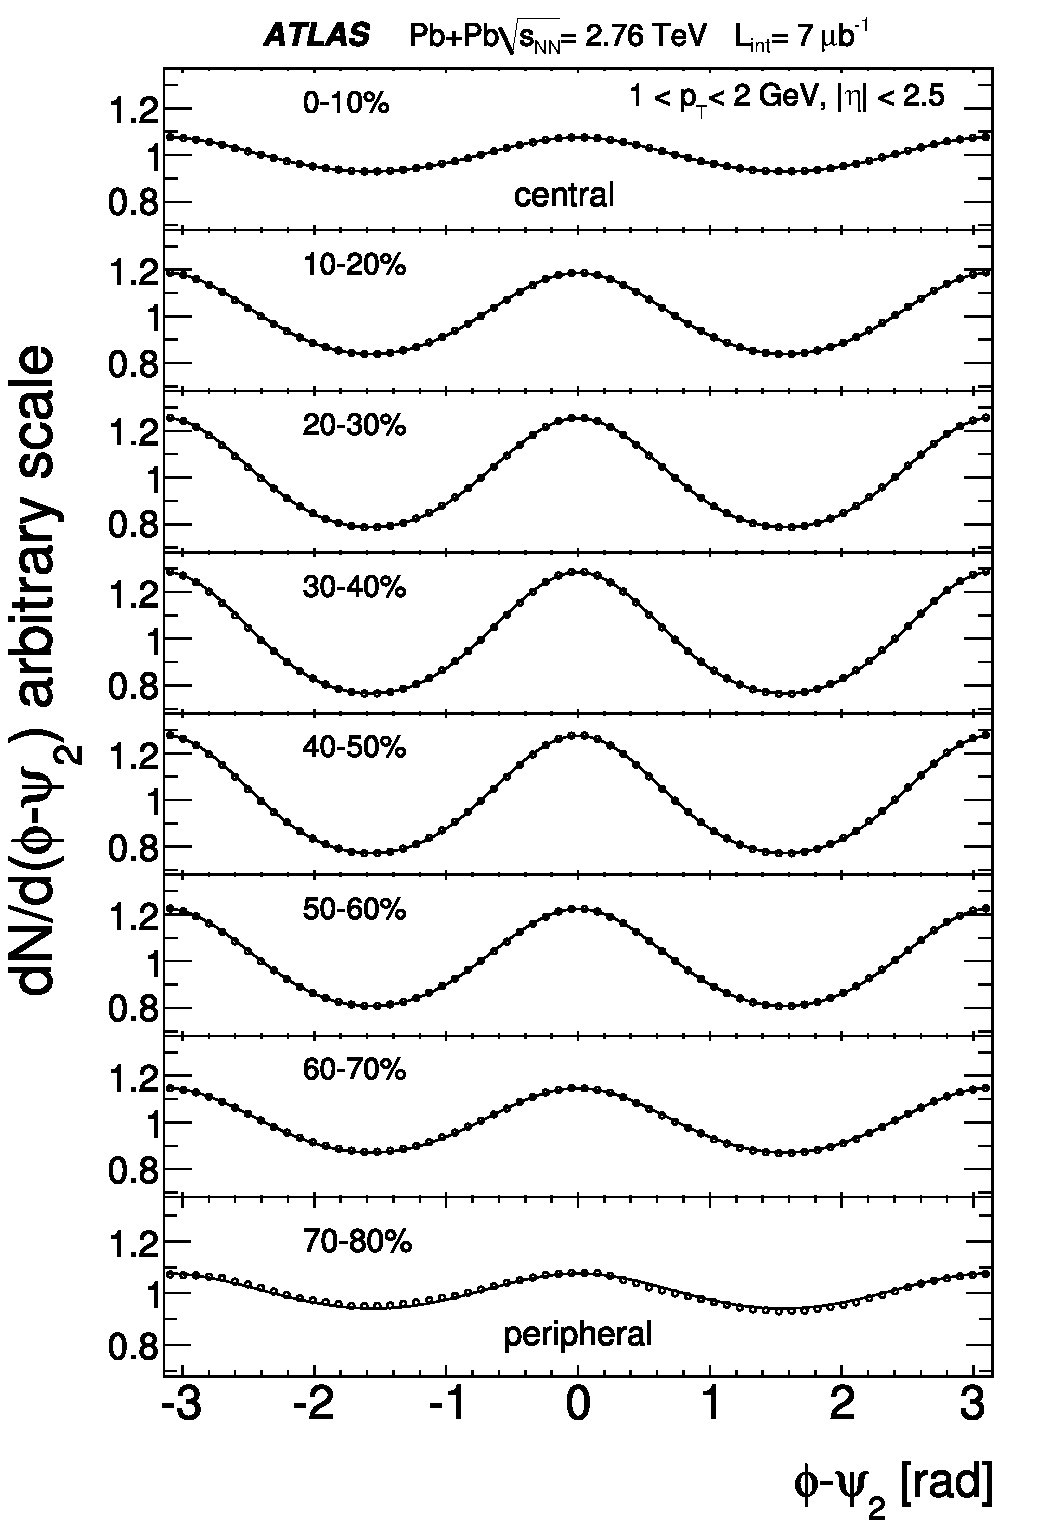
\includegraphics[width=0.49\textwidth]{flowcorrelations_figs/atlas_v2_fig_02.pdf}
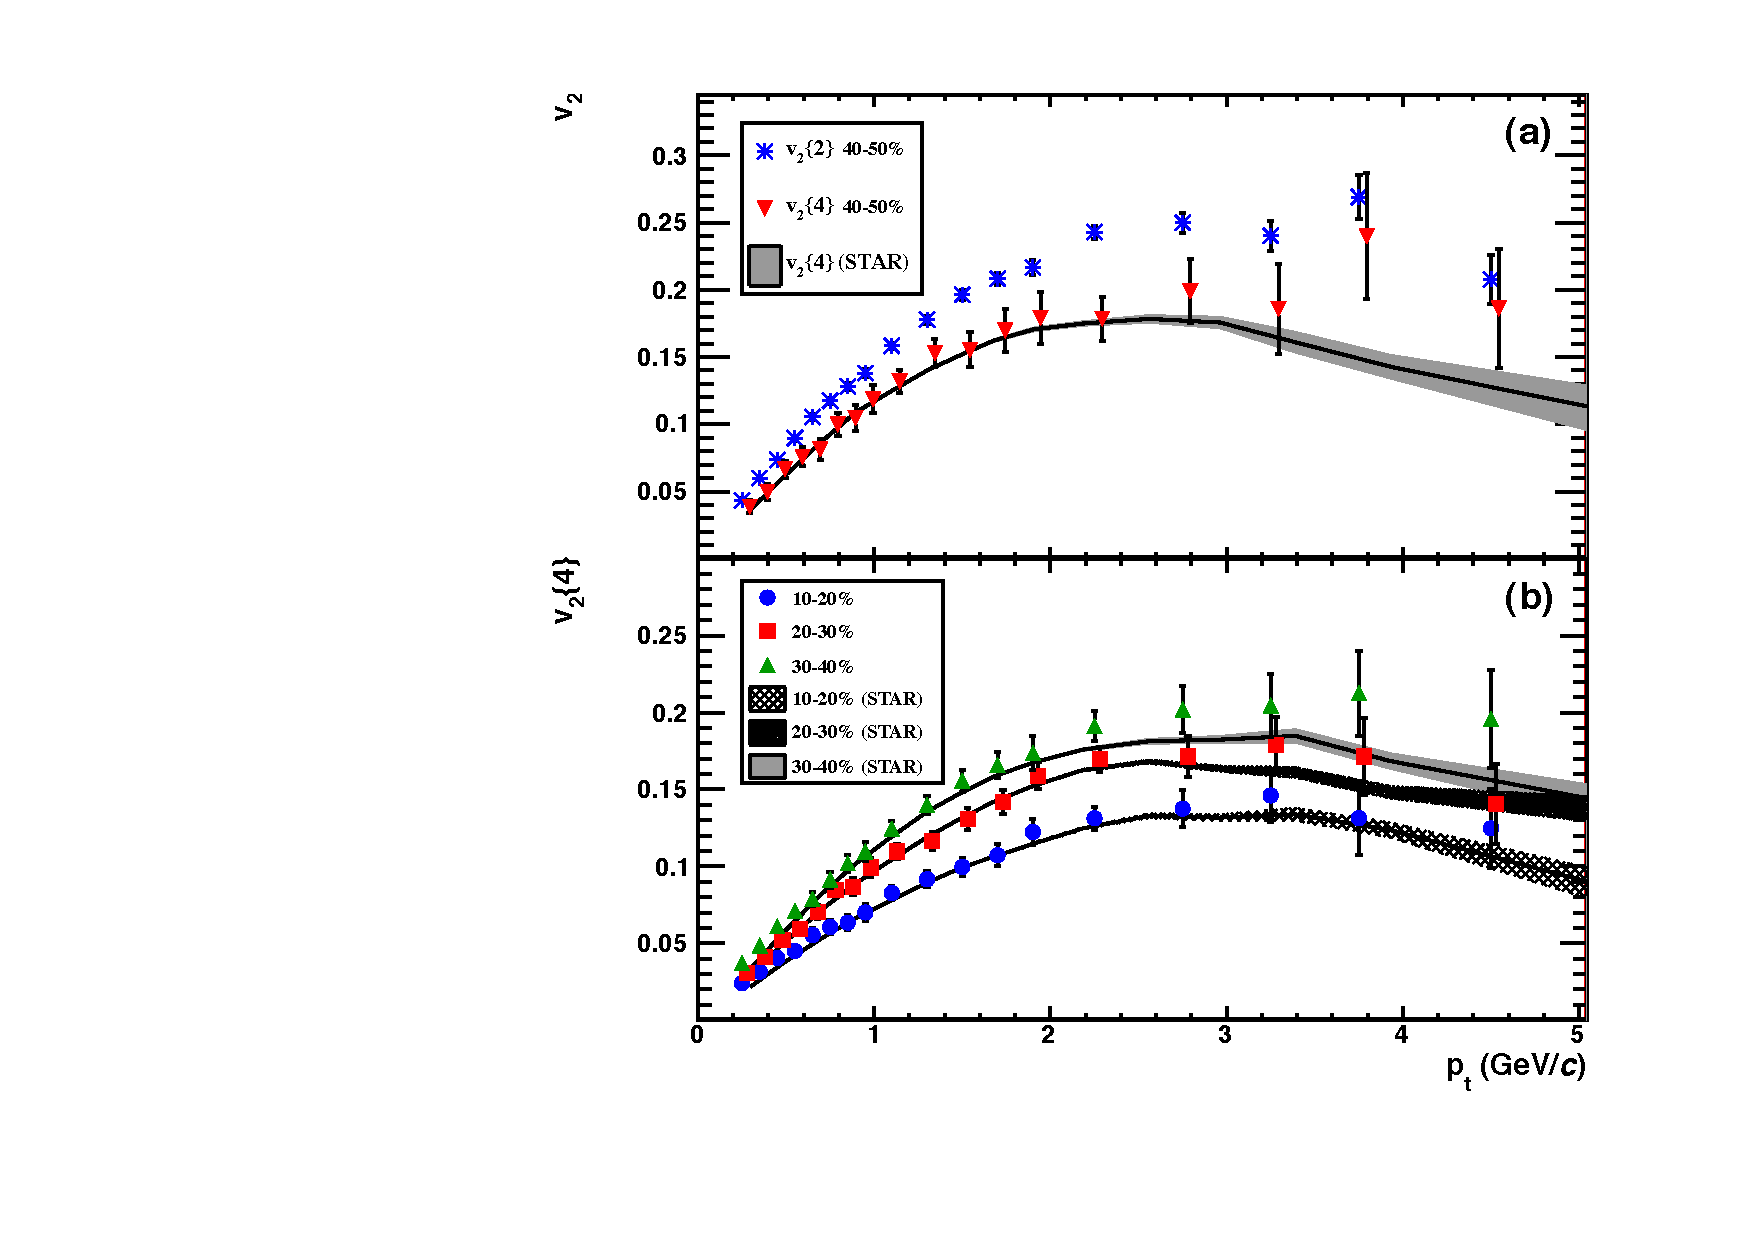
\includegraphics[width=0.49\textwidth]{flowcorrelations_figs/fig2.pdf}
\caption[]{(left) ATLAS data showing the evolution of anisotropy relative to the reaction plane, as a function of centrality (right) First ALICE data on \vtwo in Pb+Pb collisions at the LHC.}
\label{fig:pas:fc:firstreusults}
\end{center}
\end{figure}
The first LHC data on elliptic flow was released by the ALICE collaboration soon after the first collisions, 
and is shown in Figure~\ref{fig:pas:fc:firstreusults}.
The elliptic flow was estimated using three methods: 2-particle cumulants ($v_2{2}$), 4-particle cumulants ($v_2{4}$)
and Lee-Yang Zeros (LYZ).  The latter method was only used for integral flow.  
As a function of \pT, the magnitude of $\v_2$ was found to be quantitatively very similar to that measured in
the STAR experiment at RHIC, using similar methods.

\begin{figure}[!htb]
\begin{center}
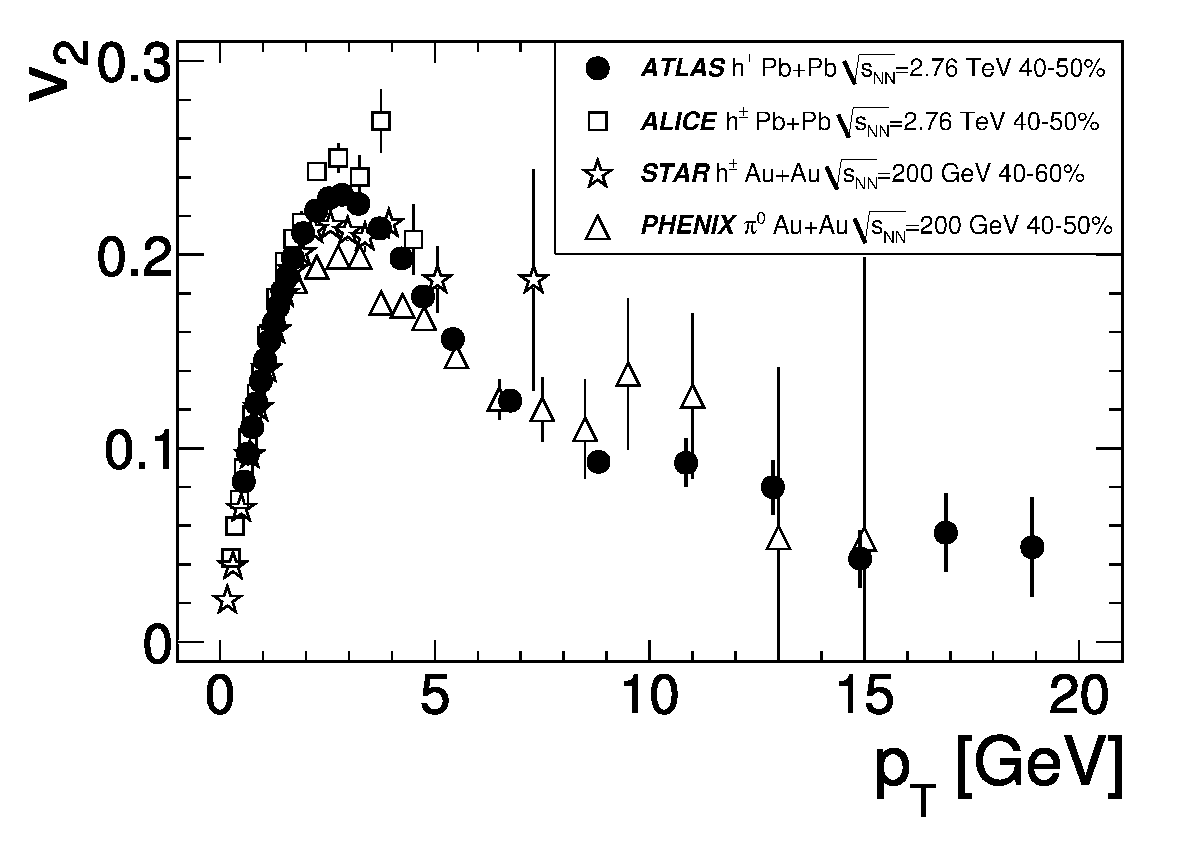
\includegraphics[width=0.49\textwidth]{flowcorrelations_figs/atlas_v2_fig_06.pdf}
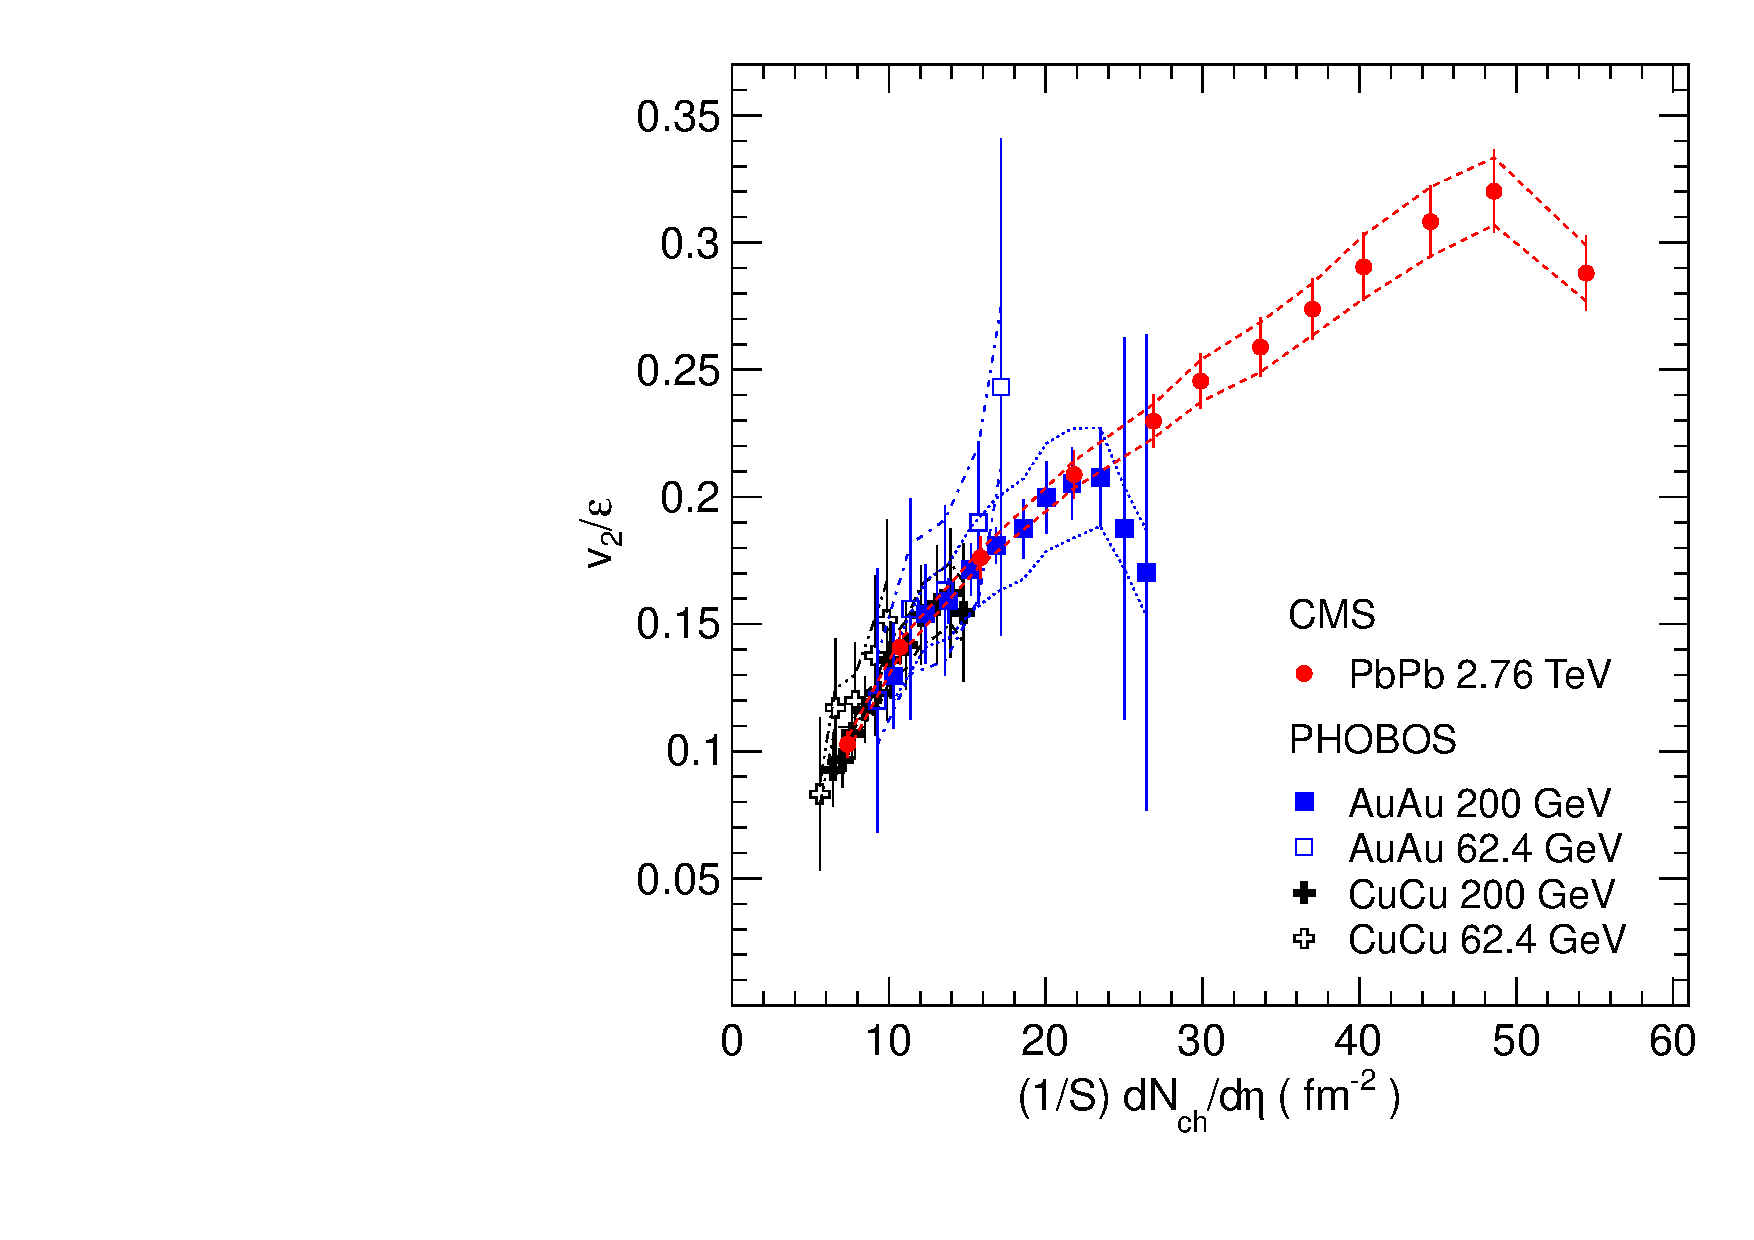
\includegraphics[width=0.49\textwidth]{flowcorrelations_figs/v2eps_dNdetaoverS_PHOBOS.pdf}
\caption[]{(left) ATLAS data showing the invariance of $\vtwo( \pT )$ with beam energy (right) CMS compilation showing the observed scaling of $\vtwo /\epsilon$ vs. $(1/S) dN_{ch}/d\eta$.}
\label{fig:pas:scaling}
\end{center}
\end{figure}

\begin{figure}[!htb]
\begin{center}
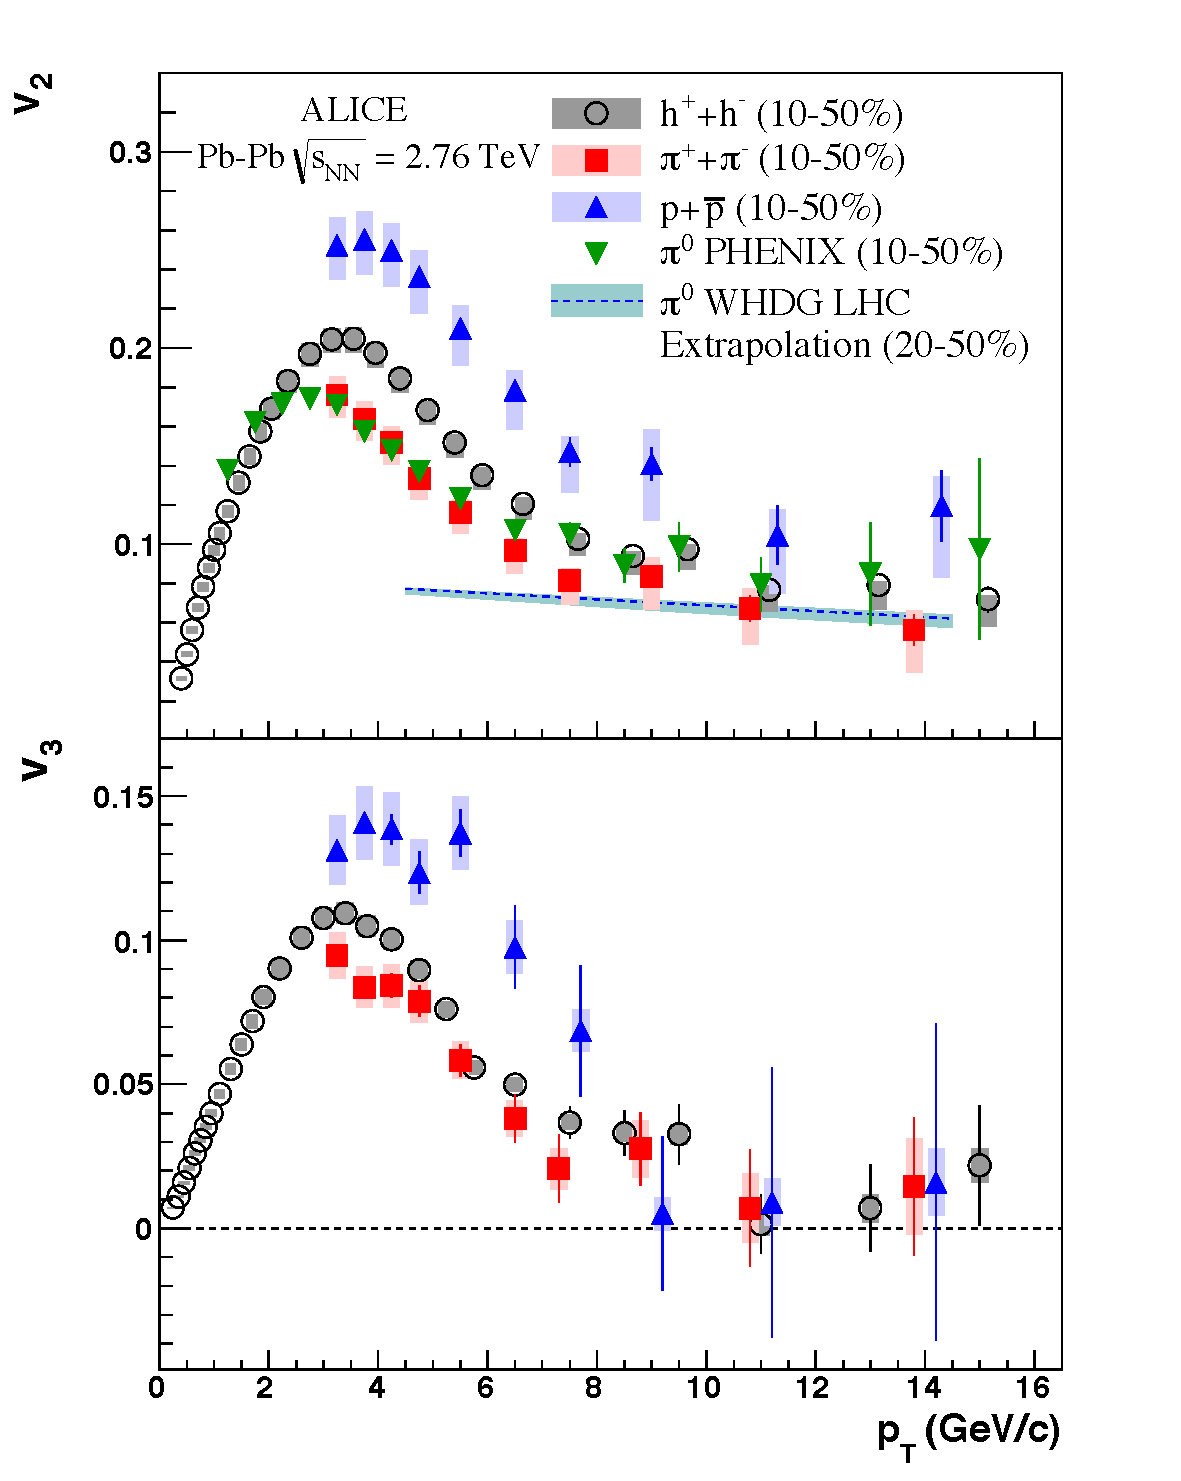
\includegraphics[width=0.49\textwidth]{flowcorrelations_figs/fig5_vn_pid.pdf}
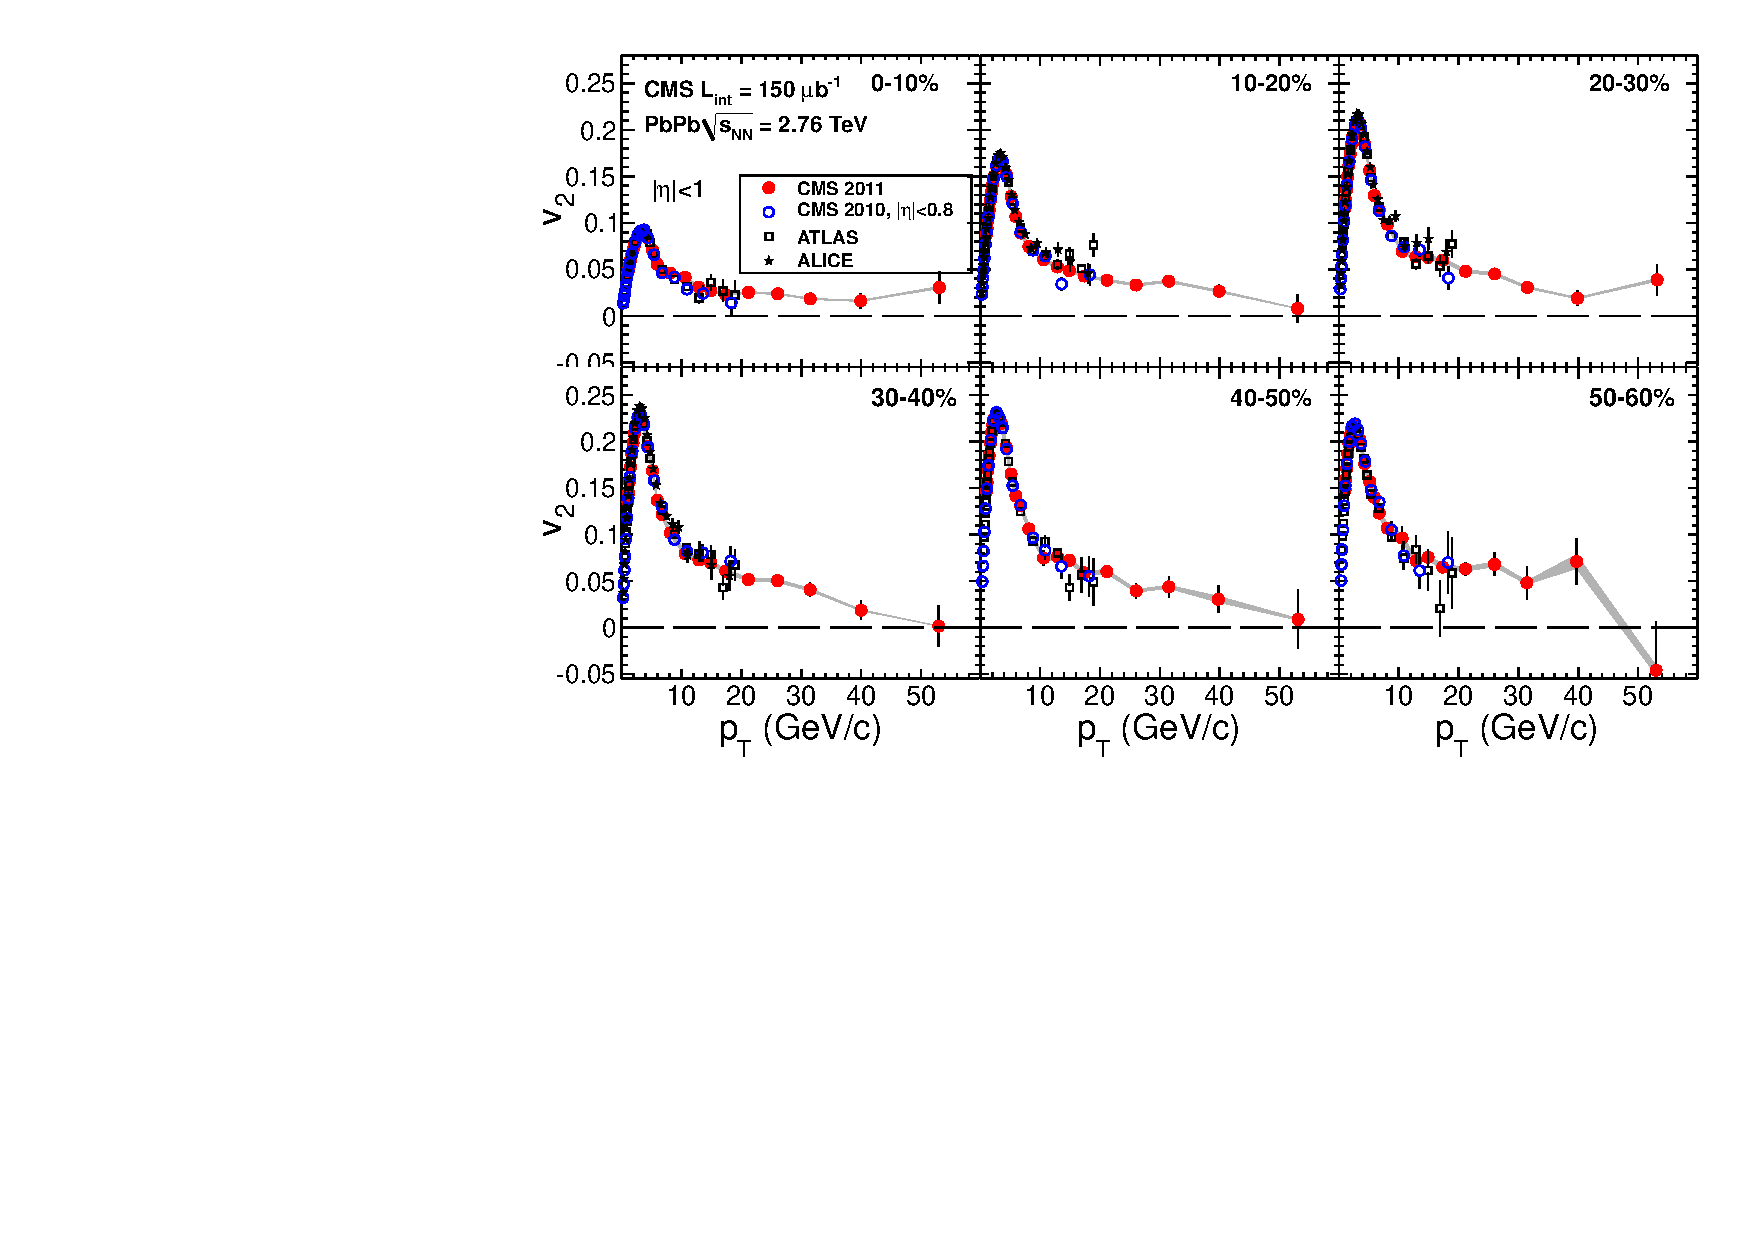
\includegraphics[width=0.49\textwidth]{flowcorrelations_figs/v2_pt_ep_atlas_alice_eta0-1_band_v5.pdf}
\caption[]{(left) ALICE data showing $\vtwo(\pT)$ for identified hadrons, for $|\eta|<0.8$ (right) CMS data showing the $\vtwo$ for unidentified hadrons at very high \pT, out to 50 GeV}
\label{fig:pas:fc:highpt}
\end{center}
\end{figure}

\begin{figure}[!htb]
\begin{center}
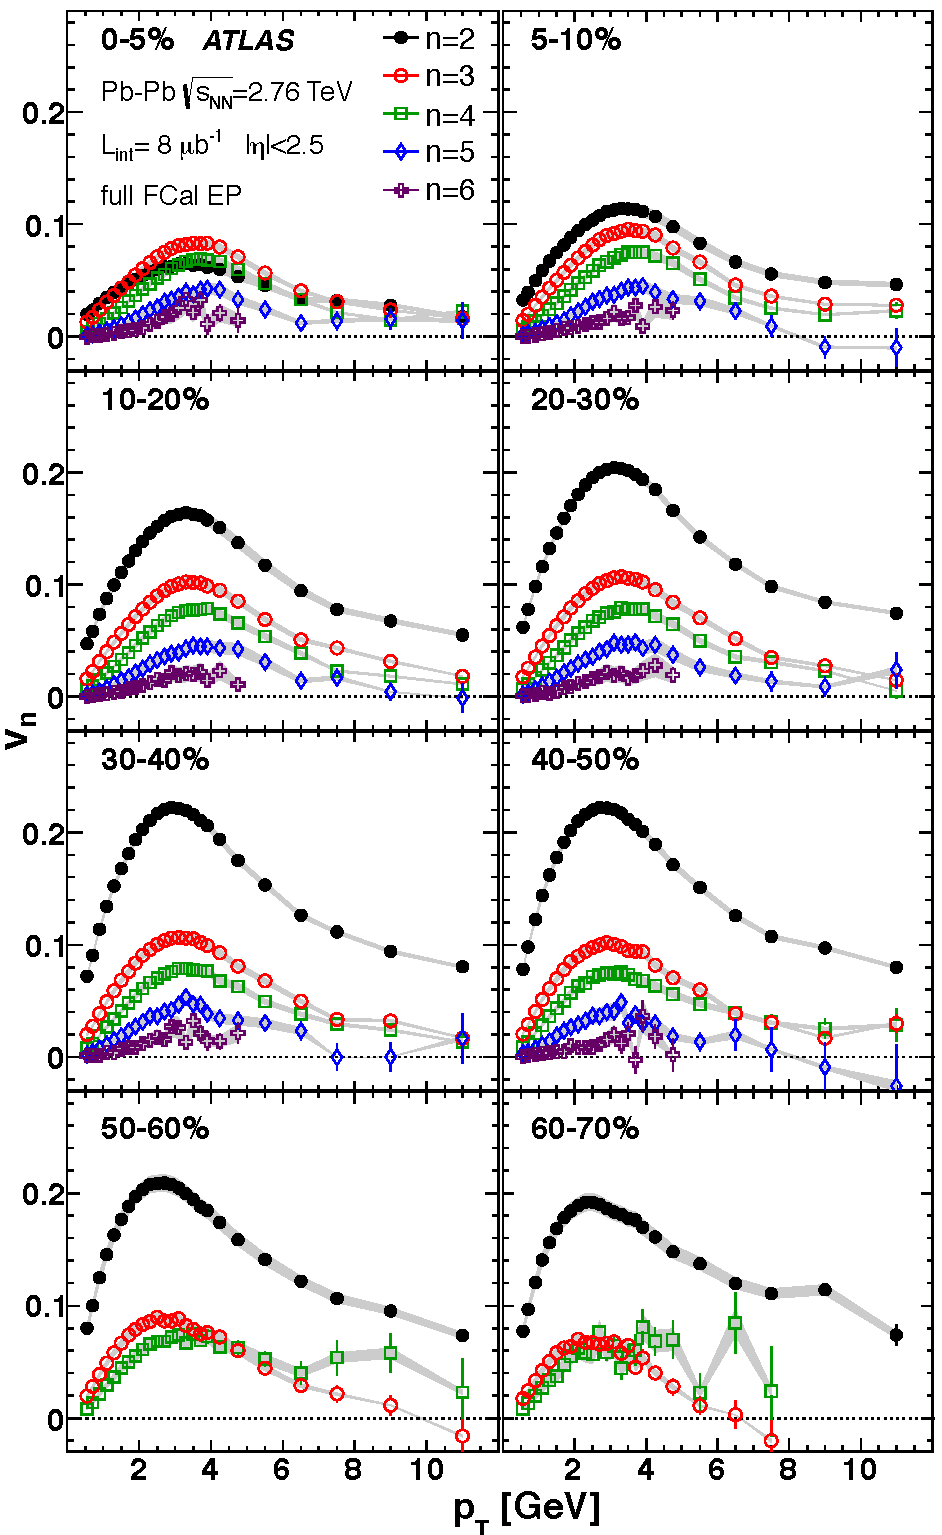
\includegraphics[width=0.49\textwidth]{flowcorrelations_figs/atlas_vn_fig_04.pdf}
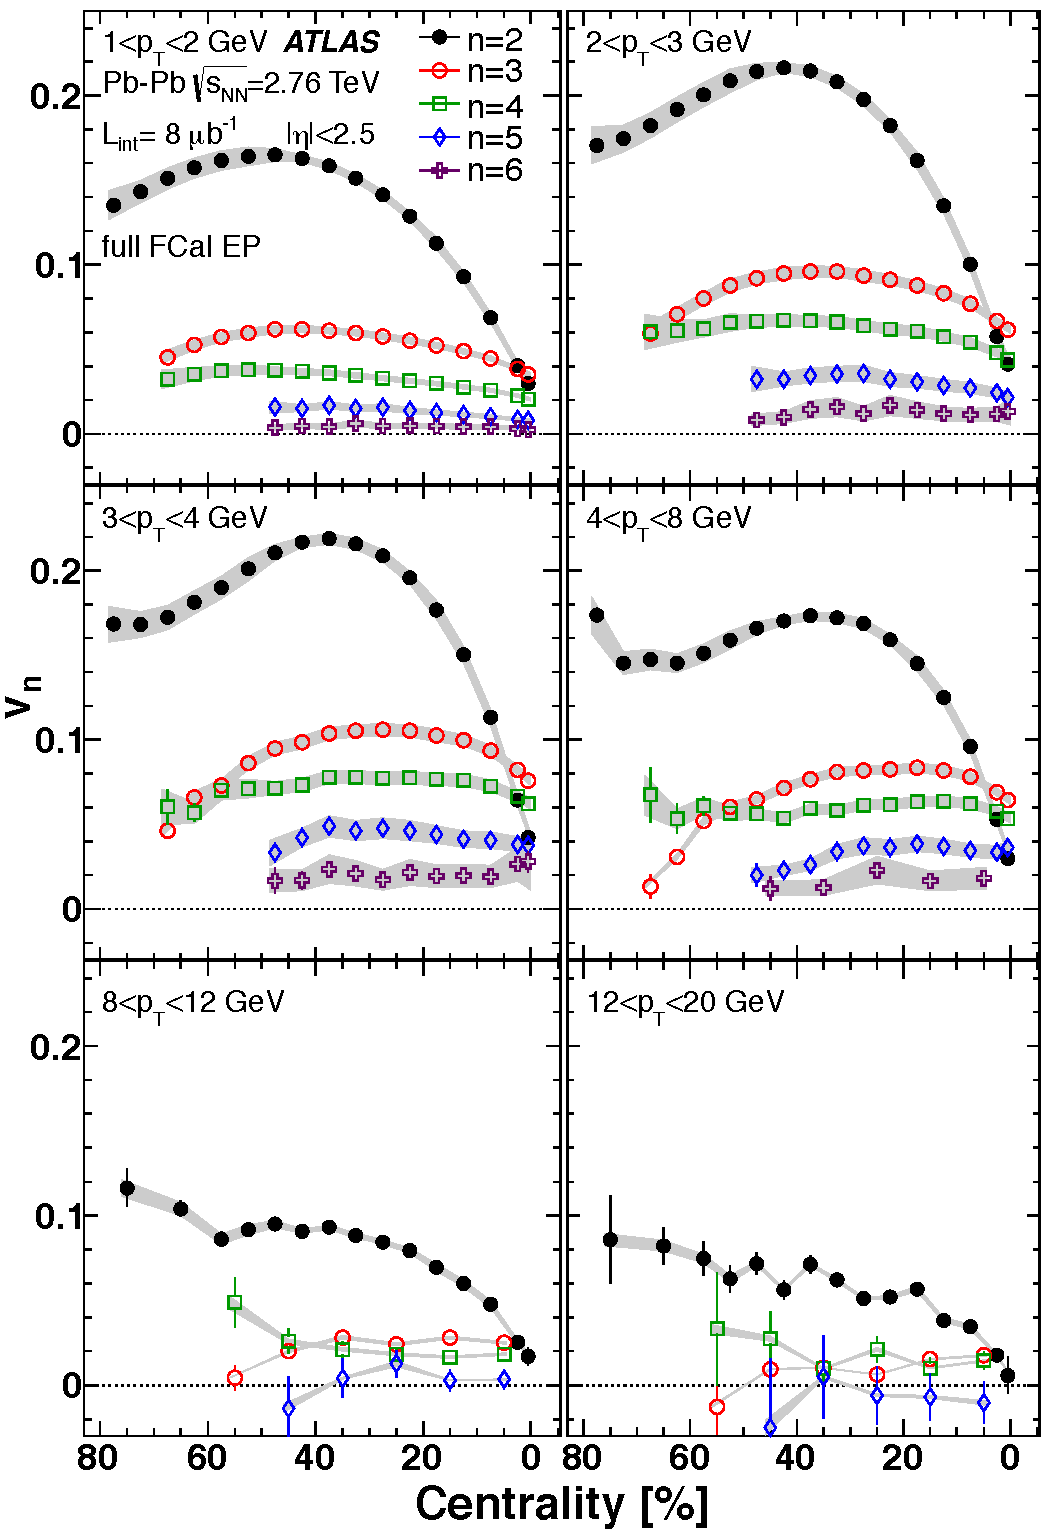
\includegraphics[width=0.49\textwidth]{flowcorrelations_figs/atlas_vn_fig_05.pdf}
\caption[]{(left) ATLAS data showing $v_n(\pT)$ for different centrality intervals and $|\eta|<2.5$, for $n=2-6$.  Very little dependence on $\eta$ is observed.  
(right) The same ATLAS data, in \pT intervals, showing the centrality dependence of $v_n$.}
\label{fig:pas:fc:vn}
\end{center}
\end{figure}

\begin{figure}[!htb]
\begin{center}
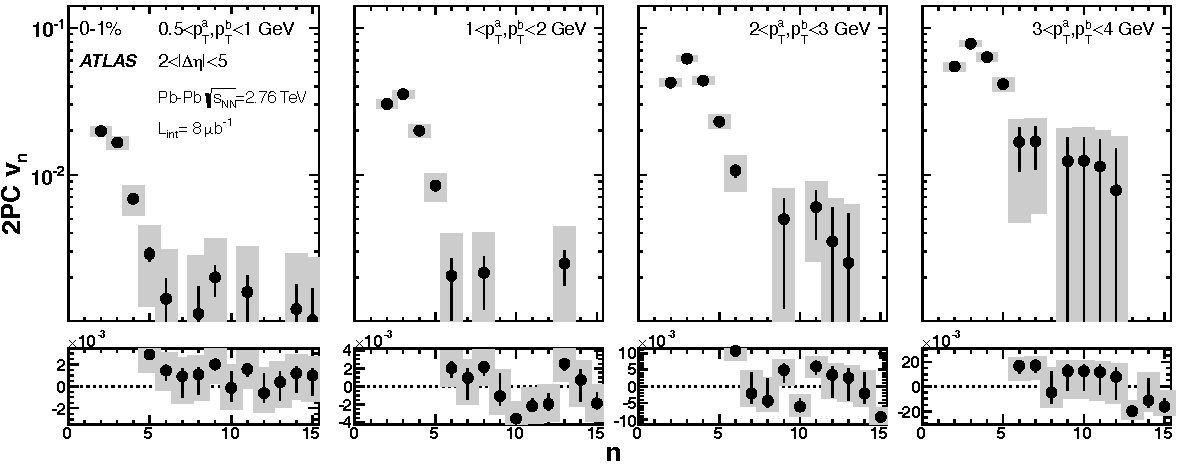
\includegraphics[width=0.98\textwidth]{flowcorrelations_figs/atlas_vn_fig_13.pdf}
\caption[]{
ATLAS data showing the $n$ dependence of $v_n$ in four \pT intervals, which are effectively
angular power spectra at different resolution scales.
}
\label{fig:pas:fc:powerspec}
\end{center}
\end{figure}

\begin{figure}[!htb]
\begin{center}
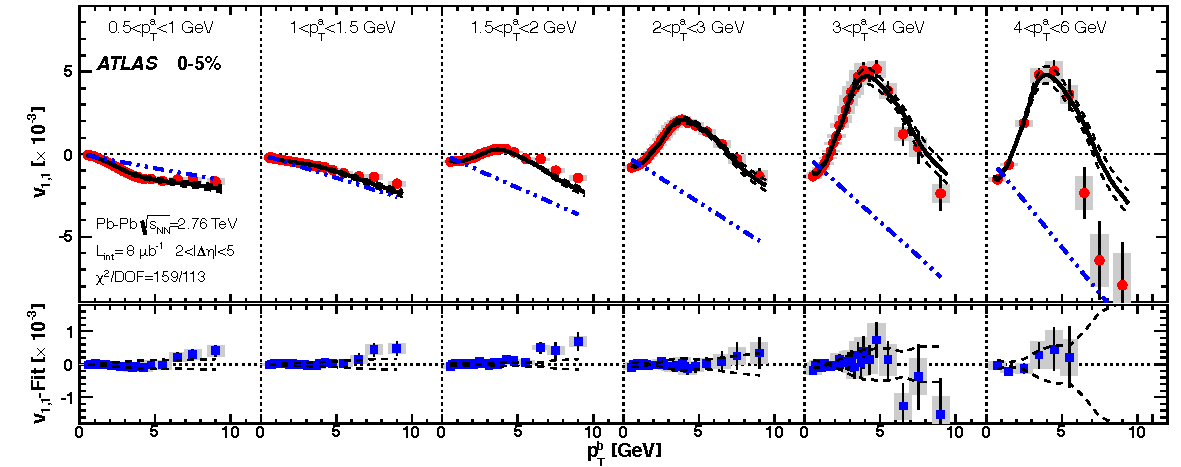
\includegraphics[width=0.98\textwidth]{flowcorrelations_figs/atlas_vn_fig_20a.pdf}
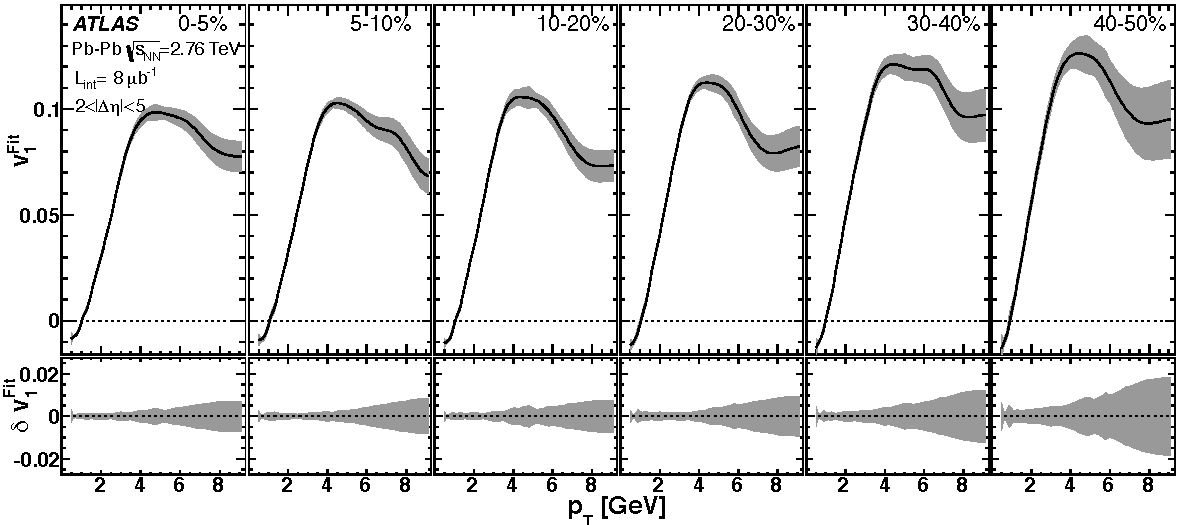
\includegraphics[width=0.98\textwidth]{flowcorrelations_figs/atlas_vn_fig_21.pdf}
\caption[]{
(top) ATLAS data showing the amplitude of $v_{1,1}$ the dipole modulation in the 2-particle correlation function, as a function of $p^b_T$ for ranges in $p^a_T$.  The fit used to extract the functional form of $v_1(\pT)$ is shown.
(bottom) The extracted functional form of $v_1(\pT)$, from the fits shown above, as a function of centrality.
}
\label{fig:pas:fc:v1}
\end{center}
\end{figure}

\begin{figure}[!htb]
\begin{center}
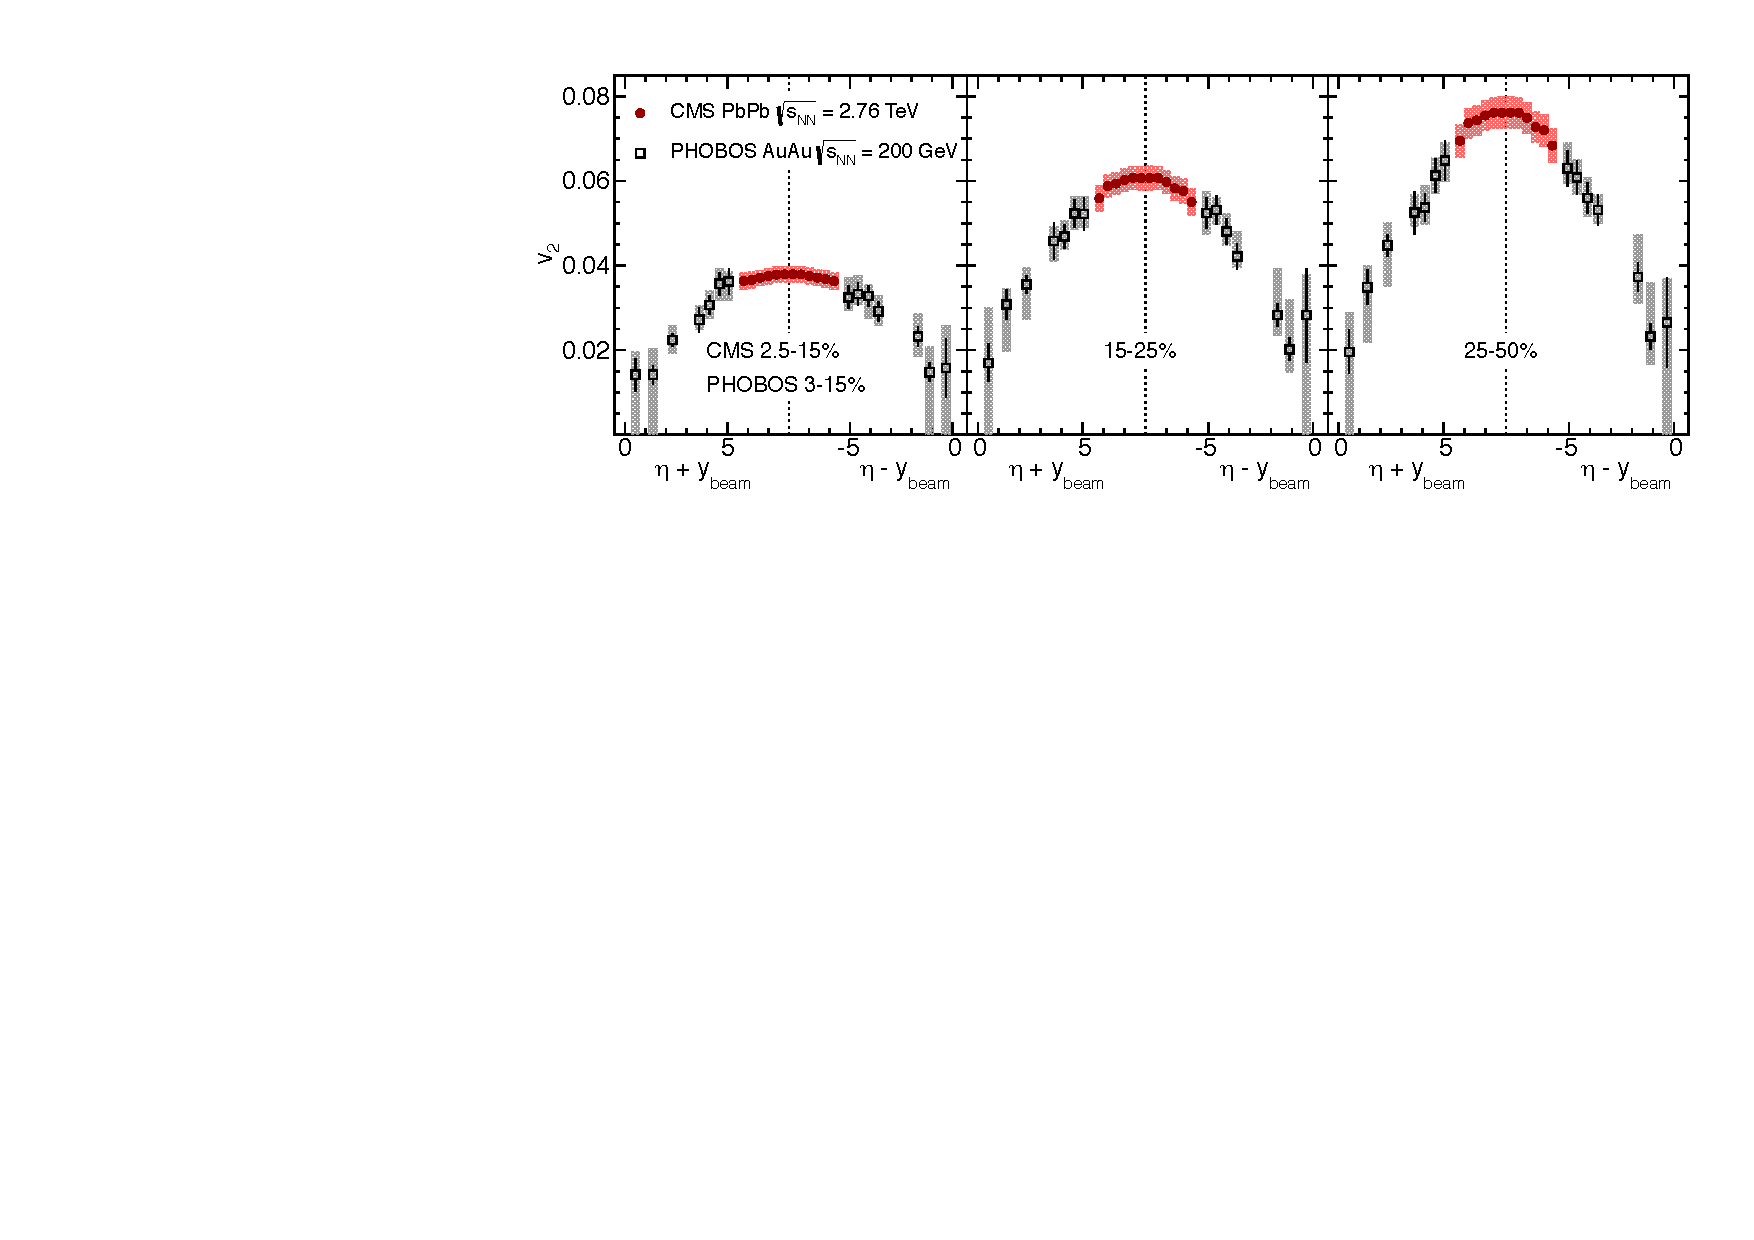
\includegraphics[width=0.98\textwidth]{flowcorrelations_figs/v2_etashifted_3cen_PHOBOS.pdf}
\caption[]{
CMS data showing $\vtwo$ for unidentified hadrons as a function of $\eta - y_{\mathrm{beam}}$, averaged over $0 <\pT < 3$ GeV (using an extrapolation procedure to cover $\pT <300$ Mev).
Results are compared to data from $\sqrt{s_{NN}}=200$ GeV
at large $\eta$ from the PHOBOS experiment at RHIC.
}
\label{fig:pas:fc:limfrag}
\end{center}
\end{figure}

\begin{figure}[!htb]
\begin{center}
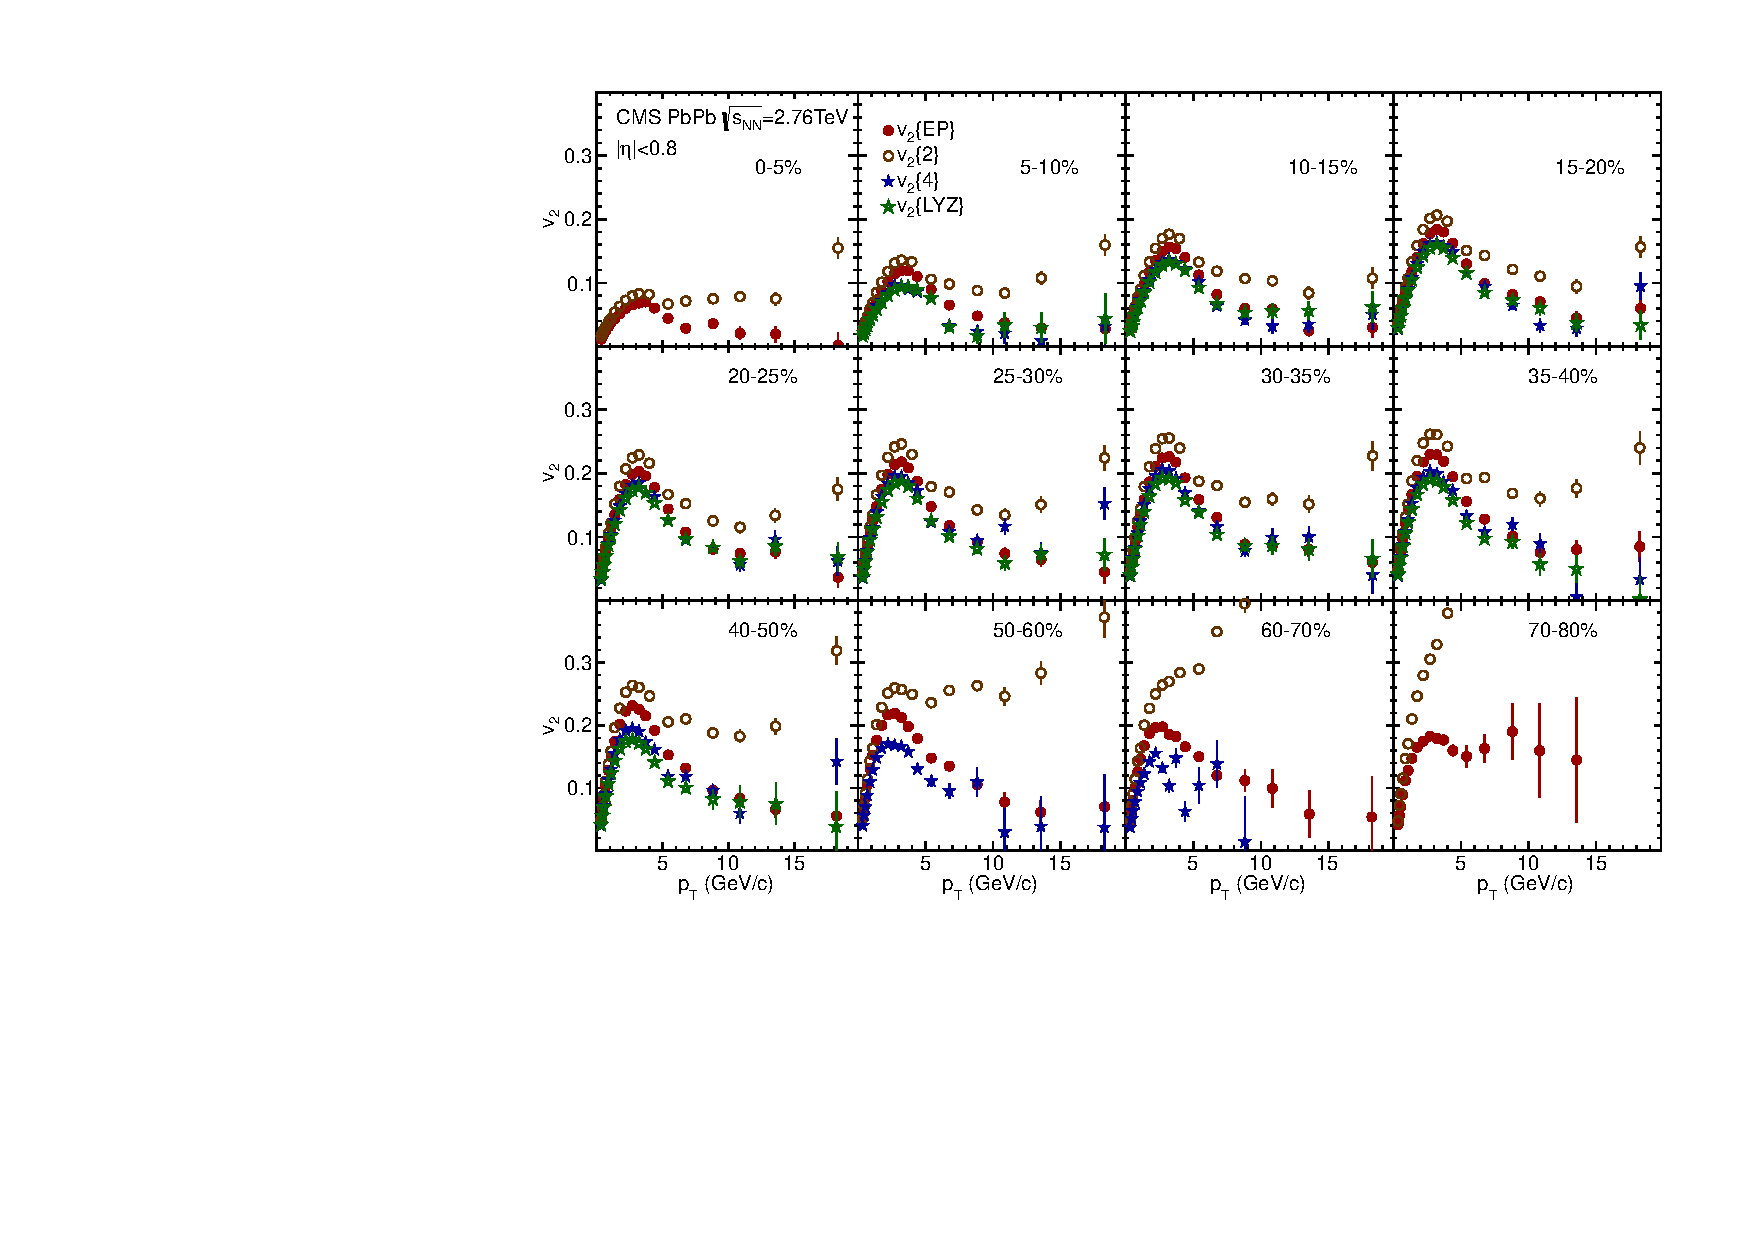
\includegraphics[width=0.98\textwidth]{flowcorrelations_figs/v2_pt_12cen_4methods.pdf}
\caption[]{
CMS data showing $\vtwo(\pT)$ in centrality intervals, using four different methods of extracting
$\vtwo$: event plane (EP), 2-particle cumulants, 4-particle cumulants, and Lee-Yang Zeros.
}
\label{fig:pas:fc:methods}
\end{center}
\end{figure}



